\documentclass[brazil,times]{abnt}
\usepackage[T1]{fontenc}
\usepackage[utf8]{inputenc}
\usepackage[pdfborder={0 0 0}]{hyperref}
\makeatletter
\usepackage{babel}
\makeatother
\usepackage{graphicx}
\begin{document}

\autor{Pedro Paulo Vezzá Campos \\ Rafael Elias Pedretti
\\ Juarez Angelo Piazza Sacenti}

\titulo{Documento de Requisitos - Iteração 1}

\comentario{Trabalho apresentado para avaliação na disciplina INE5417, do curso
de Bacharelado em Ciências da Computação, turma 04208, da Universidade Federal
de Santa Catarina, ministrada pela professora Patrícia Vilain}

\instituicao{Departamento de Informática e Estatística \par Centro
Tecnológico\par Universidade Federal de Santa Catarina}

\local{Florianópolis - SC, Brasil}

\data{25 de agosto de 2010}

\capa

\folhaderosto

\tableofcontents

\chapter{Perfil do Cliente e Visão do Problema}
O LabUFSC é um dos maiores maiores laboratórios de informática da UFSC, com um
parque de 194 máquinas. Como forma de melhorar o serviço de 
suporte e manutenção dos equipamentos o laboratório demanda de um software de
help desk.

Espera-se do software que ele seja capaz de permitir que um usuário registre um
pedido de suporte através de uma interface denominada “Front-end”. Tal pedido
será registrado em uma interface restrita à equipe de manutenção, o “Back-end”,
que poderá tratar o problema de diferentes maneiras: Delegação (À equipe da
secretaria do laboratório), resolução remota ou presencial. Ao final do
processo um Administrador poderá marcar um problema como resolvido ou não,
adicionando informações relevantes ao problema.

O sistema deverá armazenar as ocorrências para consulta posterior pela equipe
de manutenção. Deve ser possível a geração de relatórios diversos, tais como a
evolução do número de pedidos, resoluções, tempo médio de resposta, dentre
outros.

Há, ainda, a possibilidade de um Administrador configurar o sistema para um
modo automático de operação, que consiste em armazenar e redirecionar os
pedidos de suporte para a equipe da secretaria, que tomará apenas consentimento
do problema através da interface de “Back-end Secretaria”, podendo ou não resolvê-lo.

O ecossistema é heterogêneo, composto por diversos sistemas operacionais, sendo
necessário um sistema multi-plataforma (Linux e Windows).

Não há restrições de tempo rígidas, sendo tolerável tempos de resposta do
sistema (excetuado tempo de transmissão da rede) de aproximadamente 1 segundo.

\chapter{Requisitos Funcionais}
\section{Descrição Breve dos Casos de Uso}
\begin{description}
  \item[Reportar Problema:] O usuário informa sua matrícula e uma descrição do
  problema encontrado. O Front-end tentará informar via rede o Back-end do
  pedido de suporte. Em caso de sucesso, o pedido é registrado no Back-end. O
  Front-end então informa o usuário do sucesso ou fracasso da notificação.
  \item[Verificar Novos Problemas:] O Administrador verifica o Back-end em
  busca de pedidos pendentes de suporte. Ao encontrá-los pode utilizar
  diferentes abordagens: Assistência remota, presencial ou delegação.
  \item[Gerar Relatório:] O Administrador pode gerar relatórios tais como a
  evolução do número de pedidos, resoluções, tempo médio de resposta através dos
  dados coletados nos últimos 30 dias.
  \item[Delegar Problema:] Especifica o funcionamento do ato de delegação de
  tarefas de um Administrador para um Atendente. Caso de uso incluso no caso
  ``Verificar Novos Problemas''.
  \item[Receber Delegação:] Contraparte do caso de uso anterior, apresentando a
  perspectiva do Atendente ao receber uma delegação de atendimento de um
  Administrador.
  \item[Adicionar Usuário:] Explica o funcionamento da função de adição de novos
  usuários no sistema.
  \item[Remover Usuário:] Explica o funcionamento da função de remoção usuários
  do sistema.
  \item[Alterar Usuário:] Explica o funcionamento da função de alteração de
  dados de usuários do sistema.
  \item[Acessar Remotamente:] Especifica o funcionamento do ato de um
  Administrador acessar remotamente e enviar comandos a uma máquina utilizando o
  Back-end.
  \item[Configuração de Modo Automático:] Em caso de ausência de um
  Administrador no local, especifica um funcionamento especial do sistema, realizando
  delegações automáticas aos Atendentes.
  \item[Recebimento de Delegação em Modo Automático:] Apresenta a perspectiva de
  funcionamento do Back-end Secretaria em caso de acionamento do modo
  automático.
\end{description}

\subsection{Cronograma de implementação dos casos de uso}
Para a Iteração 1 estão planejados todos os casos de uso descritos
anteriormente, à exceção dos dois últimos, que foram alocados para a Iteração 2.

\section{Diagrama de Casos de Uso}
%\usepackage{graphics} is needed for \includegraphics
\begin{figure}[htp]
\begin{center}
  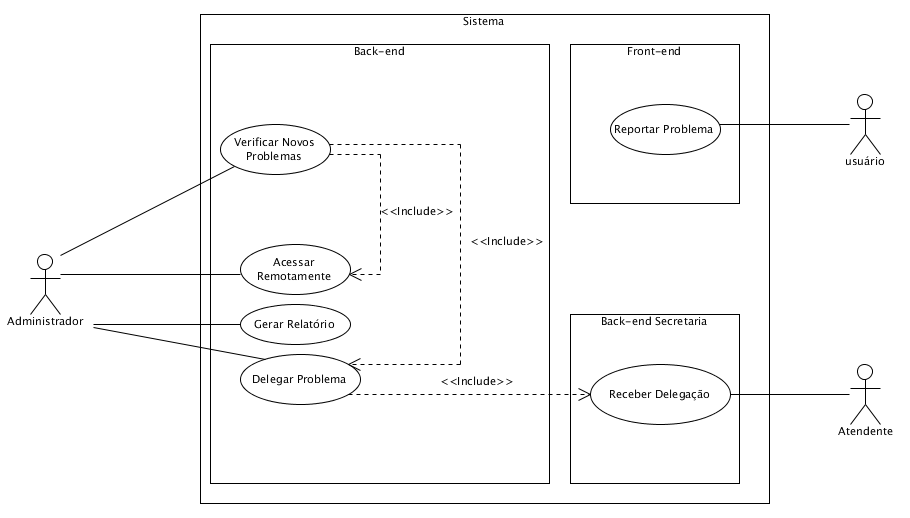
\includegraphics[width=\linewidth]{diagramas/diagramaDeUso.png}
  \caption[Diagrama de Casos de Uso da Iteração 1]{Diagrama de Casos de Uso da Iteração 1}
  \label{diagrama-casos-uso}
\end{center}
\end{figure}

\newpage

\section{Diagrama de Classes Conceituais}
%\usepackage{graphics} is needed for \includegraphics
\begin{figure}[htp]
\begin{center}
  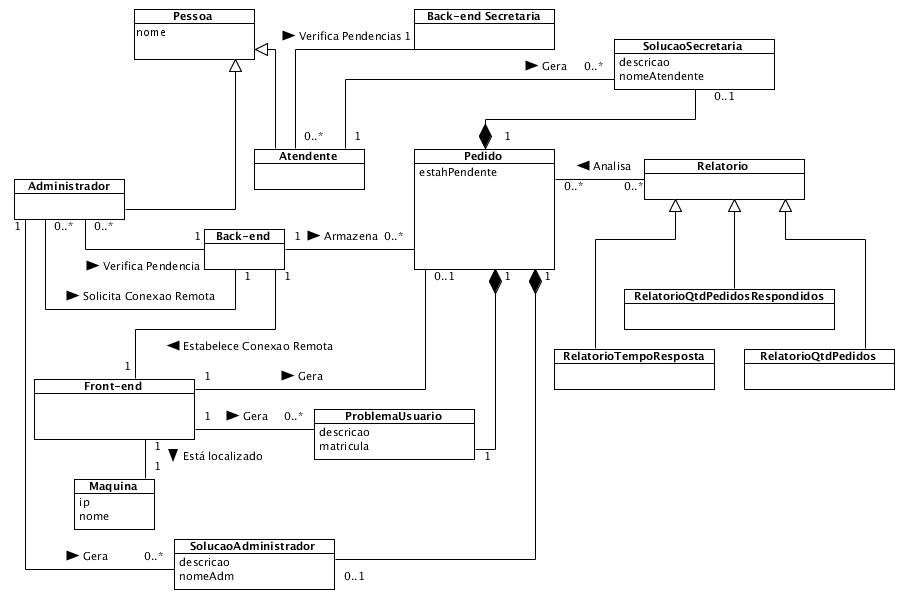
\includegraphics[width=\linewidth]{diagramas/diagramaConceitual.png}
  \caption[Diagrama de classes conceituais para os casos de uso
  da Iteração 1]{Diagrama de classes conceituais para os casos de uso
  da Iteração 1}
  \label{diagrama-conceitual}
\end{center}
\end{figure}


\section{Front-end: Reportar Problema}
\begin{description}
\item[Escopo:] Sistema Front-end
\item[Nível:] Meta do usuário
\item[Ator Primário:] Usuário

\item[Stakeholders e seus interesses:] \hfill \\ 
Usuário: Deseja que seu pedido de suporte seja recebido e atendido

\item[Pré-condições:] O sistema e a rede estão operantes. O aluno possui
matrícula válida (segundo regras descritas na Especificação Suplementar).

\item[Pós-condições:] É emitida uma notificação para o usuário.

\item[Fluxo Básico ou Cenário Principal:] \hfill
\begin{enumerate}
  \item O usuário acessa o Front-end
  \item O usuário informa sua matrícula e uma breve descrição do seu problema.
  \item O usuário submete as informações.
  \item O sistema informa o usuário do sucesso do envio.
  \item O usuário é atendido e seu problema é resolvido.
\end{enumerate}

\item[Extensões:] \hfill
\begin{description}
	\item[*a.] A qualquer momento, o sistema ou a rede falha:
		\begin{enumerate}
 			\item O sistema informa o usuário da incapacidade de envio e sugere chamar    
  			pessoalmente um Atendente.
  			\item  O sistema tenta periodicamente reestabelecer a conexão.
		\end{enumerate}

	\item[2a.] Matrícula inválida ou descrição em branco:
	\begin{enumerate}
		\item  O sistema sinaliza o erro e rejeita a entrada.
	\end{enumerate}
\end{description}
\item[Requisitos especiais:] Nenhum

\item[Tecnologia:] \hfill
\begin{description} 
	\item[2a.] A entrada dos dados é feita pelo teclado.
	\item[4a.] O sistema informa o usuário por meio do monitor.
\end{description}
\item[Freqüência de Ocorrência:] Raramente.

\end{description}



\section{Back-end: Verificar Novos Problemas}
\begin{description}
\item[Escopo:] Sistema Back-end
\item[Nível:] Meta do Administrador
\item[Ator Primário:] Administrador
\item[Stakeholders e seus interesses:] \hfill \\
Administrador: Deseja ser notificado de novos pedidos e que os pedidos
sejam registrados.
\item[Pré-condições:] O sistema e a rede estão operantes. Há, pelo menos, um pedido 
pendente.
\item[Pós-condições:]  É emitida uma notificação ao Administrador e o pedido é        
registrado no Back-end.
\item[Fluxo Básico ou Cenário Principal:]\hfill
\begin{enumerate}
  \item O Administrador localiza no Back-end um pedido pendente.
  \item O Administrador analisa o problema e aciona o sistema de resolução
  remota.
  \item \emph{Há a execução do caso de uso descrito na seção \ref{Acessar-Remotamente}}
  \item O problema é resolvido pelo Administrador.
  \item O Administrador anota a solução empregada.
  \item O Administrador marca o problema como resolvido.
  \item O Back-end deve armazenar o problema do usuário, a resposta proposta e
  o Administrador que resolveu o problema.
  \item O Administrador recebe uma notificação de armazenamento da solução.
  \item \emph{Repete os passos de 1 a 8 enquanto houver pedidos pendentes.}
\end{enumerate}

\item[Extensões:]\hfill
\begin{description}
	\item[*a.] A qualquer momento, o sistema ou a rede falha: \hfill
	\begin{enumerate}
 		\item A rede deve ser reestabelecida e o sistema
 		reiniciado manualmente.
	\end{enumerate} 

	\item[2a.] O Administrador decide fazer atendimento presencial:
	\begin{enumerate}
  		\item O Administrador resolve localmente o problema.
	\end{enumerate}

	\item[2b.] O Administrador delega o problema à secretaria:
	\begin{enumerate}
  		\item \em{É executado o caso de uso descrito na seção
  		\ref{delegar-problema}}
	\end{enumerate}

	\item[3a.] O problema é resolvido pela Secretaria:
	\begin{enumerate}
  		\item A secretaria notifica o Administrador da resolução do problema.
	\end{enumerate}

	\item[3b.] O problema não é resolvido pela Secretaria:
	\begin{enumerate}
  		\item A secretaria notifica o Administrador da não resolução do problema.
	\end{enumerate}

	\item[(4-7)a.] O problema não foi resolvido:
	\begin{enumerate}
  		\item O problema continua como pendente até ser resolvido.
	\end{enumerate}
\end{description}

\item[Requisitos especiais:] Dispositivo de aviso sonoro.
\item[Tecnologia:] Nenhuma.
\item[Freqüência de Ocorrência:] Regular.

%\usepackage{graphics} is needed for \includegraphics
\begin{figure}[htp]
\begin{center}
  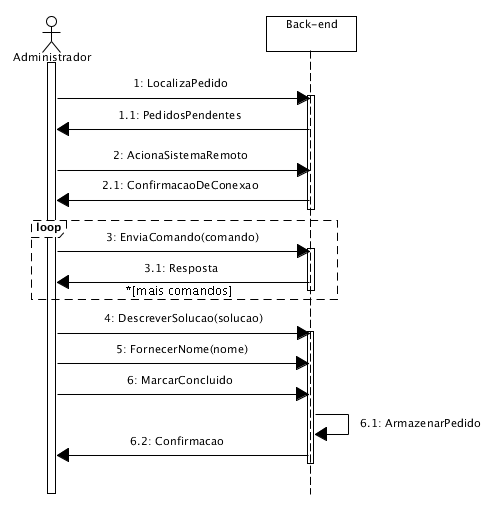
\includegraphics[scale=0.65]{diagramas/diagramaDeSequenciaProblema.png}
  \caption[Diagrama de sequência do sistema para verificar novos problemas
  ]{Diagrama de sequência do sistema para verificar novos problemas}
  \label{diagrama-sequencia-problema}
\end{center}
\end{figure}
\item[Contrato:] EnviaComando
\begin{description}
  \item[Operação:] EnviaComando(comando)
  \item[Referências cruzadas:] caso de uso Verificar Novos Problemas
  \item[Pré-condições:] \hfill
  	\begin{itemize}
  		\item O sistema e a rede estão operantes;
  		\item O Front-end remoto está conectado ao Back-end;
  		\item \underline{comando} é uma instrução válida, executável pelo Front-end
  		remoto.
	\end{itemize}
  \item[Pré-condições:] \hfill
  	\begin{itemize}
  		\item O comando foi executado;
  		\item As informações retornadas pelo comando são fornecidas ao Back-end;
	\end{itemize}
\end{description}

\end{description}


\section{Back-end: Gerar Relatório}
\begin{description}
\item[Escopo:] Sistema Back-end
\item[Nível:] Meta do Administrador
\item[Ator Primário:] Administrador
\item[Stakeholders e seus interesses:] \hfill \\
Administrador: Deseja obter de maneira fácil relatórios que permitam coletar
estatísticas sobre os pedidos de suporte.

\item[Pré-condições:] O sistema está operante e o Administrador realizou o \emph{login}
no Back-end
\item[Pós-condições:]  É gerado o relatório requisitado pelo Administrador.
\item[Fluxo Básico ou Cenário Principal:]\hfill
\begin{enumerate}
  \item O Administrador informa o relatório desejado. As possibilidades de
  relatórios são: Número de pedidos, número de resoluções, tempo médio de
  resposta.
  \item O Back-end gerará o relatório pedido tendo como período de coleta os
  últimos 30 dias.
\end{enumerate}

\item[Extensões:]\hfill
\begin{description}
	\item[*a.] A qualquer momento, o sistema falha: \hfill
	\begin{enumerate}
 		\item O sistema deve ser reiniciado manualmente.
 		\item O Administrador deve informar suas credenciais novamente.
	\end{enumerate} 
\end{description}
\item[Requisitos especiais:] Nenhum.
\item[Tecnologia:] O relatório será gerado em formato de texto puro.
\item[Freqüência de Ocorrência:] Raramente.

\end{description}



\section{Back-end: Delegar Problema}\label{delegar-problema}
\begin{description}
\item[Escopo:] Sistema Back-end
\item[Nível:] Meta do Administrador
\item[Ator Primário:] Administrador
\item[Stakeholders e seus interesses:] \hfill \\
Administrador: Deseja delegar uma resolução de um pedido pendente à Secretaria.

\item[Pré-condições:] O sistema e a rede estão operantes e o Administrador
realizou o \emph{login} no Back-end. Há pelo menos um pedido
pendente.

\item[Pós-condições:] O Administrador confirmou a solução do problema e encerrou
o pedido.
\item[Fluxo Básico ou Cenário Principal:]\hfill
\begin{enumerate}
  \item O Administrador seleciona e envia o pedido pendente a ser delegado à
  Secretaria.
  \item \emph{Há a execução do caso de uso descrito na seção
  \ref{caso-receber-delegacao}}
  \item O Administrador recebe a resposta enviada por um Atendente através do
  Back-end Secretaria.
  \item O Administrador confirma a solução do pedido e encerra-o.
  \item O Back-end deve armazenar a confirmação de recebimento, a resposta
  do problema proposta e o Atendente que resolveu o problema. O pedido de
  suporte permanece pendente até um Administrador confirmar a solução do Atendente.
\end{enumerate}

\item[Extensões:]\hfill
\begin{description}
	\item[1a.] A delegação não foi enviada para a Secretaria.
	\begin{enumerate}
		\item O Administrador é notificado da impossibilidade de envio.
		\item O problema permanece como pendente.
	\end{enumerate}

	\item[2a.] A delegação não foi respondida pela Secretaria.
	\begin{enumerate}
 		\item O problema permanece como pendente.
	\end{enumerate}
		
	\item[4a.] O Administrador não confirma a resolução do problema. 
	\begin{enumerate}
 		\item O problema permanece como pendente.
	\end{enumerate} 
\end{description}
\item[Requisitos especiais:] Nenhum.
\item[Tecnologia:] Nenhuma.
\item[Freqüência de Ocorrência:] Regular.
\end{description}
\newpage
%\usepackage{graphics} is needed for \includegraphics
\begin{figure}[htp]
\begin{center}
  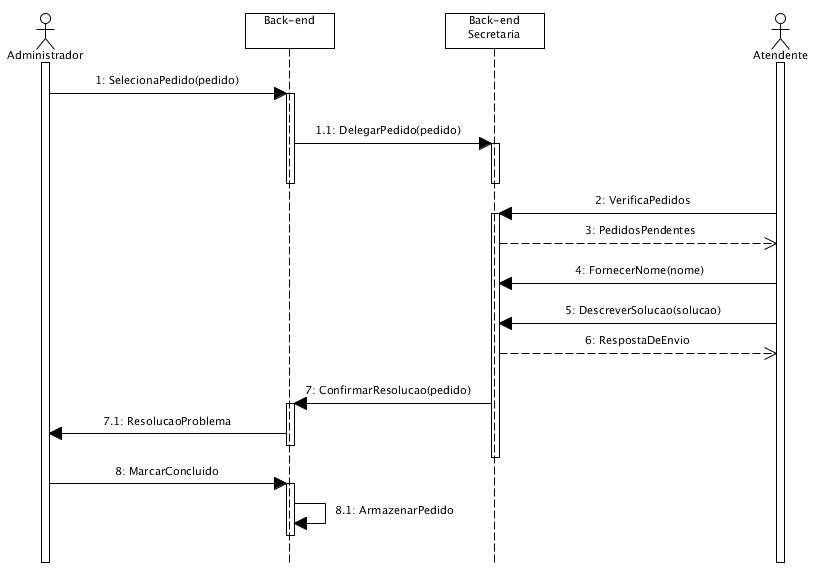
\includegraphics[scale=0.65]{diagramas/diagramaDeSequenciaDelegar.png}
  \caption[Diagrama de sequência do sistema para delegar um
  problema]{Diagrama de sequência do sistema para delegar um
  problema}
  \label{diagrama-sequencia-delegar}
\end{center}
\end{figure}



\section{Back-end Secretaria: Receber Delegação \label{caso-receber-delegacao}}
\begin{description}
\item[Escopo:] Sistema Back-end Secretaria
\item[Nível:] Meta do Atendente
\item[Ator Primário:] Atendente
\item[Stakeholders e seus interesses:] \hfill \\
Atendente: Deseja ser notificado quando houver um pedido pendente delegado por
um Administrador.

\item[Pré-condições:] O sistema e a rede estão operantes.
\item[Pós-condições:] Um Atendente recebeu um notificação de problema referente
ao pedido pendente.
\item[Fluxo Básico ou Cenário Principal:]\hfill
\begin{enumerate}
  \item O Atendente verifica pedidos pendentes.
  \item O problema é solucionado
  \item O Atendente informa a resolução.
  \item O Atendente fornece suas credenciais 
  \item O Atendente envia a resposta do problema.
  \item O Back-end Secretaria confirma o envio da resposta
  \item O Back-end deve armazenar a confirmação de recebimento, a resposta
  do problema proposta e o Atendente que resolveu o problema.
\end{enumerate}

\item[Extensões:]\hfill
\begin{description}
	\item[2a.] O Atendente não foi capaz de solucionar o problema.
	\begin{enumerate}
 		\item O Atendente informa a incapacidade de resolução.
	\end{enumerate} 
	
	\item[4a.] O Atendente fornece credenciais inválidas. 
	\begin{enumerate}
 		\item O Back-end Secretaria pede novamente as credenciais.
 		\item \emph{O passo anterior é repetido até que haja credenciais válidas.}
	\end{enumerate} 
\end{description}
\item[Requisitos especiais:] Nenhum.
\item[Tecnologia:] Nenhuma.
\item[Freqüência de Ocorrência:] Regular.

\end{description}



\section{Back-end: Adicionar Usuário}
\begin{description}
\item[Escopo:] Sistema Back-end
\item[Nível:] Meta do Administrador
\item[Ator Primário:] Administrador
\item[Stakeholders e seus interesses:] \hfill \\
Administrador: Deseja adicionar Administradores ou Atendentes.

\item[Pré-condições:] O sistema está operante. O Administrador está logado.
\item[Pós-condições:] O usuário foi adicionado.
\item[Fluxo Básico ou Cenário Principal:]\hfill
\begin{enumerate}
  \item O Administador fornece o login e senha do usuário a ser criado.
  \item O Administrador fornece o grupo do novo usuário (Administrador ou
  Atendente)
  \item A operação é executada.
\end{enumerate}

\item[Extensões:]\hfill
\begin{description}
	\item[1a.] O usuário novo já existe.
	\begin{enumerate}
 		\item O Back-end informa ao Administrador que o usuário já existe.
 		\item O Back-end requisita um novo login.
 		\item \emph{O passo anterior repete-se enquanto o usuário fornecido já
 		existir.}
	\end{enumerate}

\end{description}
\item[Requisitos especiais:] Nenhum.
\item[Tecnologia:] Nenhuma.
\item[Freqüência de Ocorrência:] Raramente.

\end{description}



\section{Back-end: Remover Usuário}
\begin{description}
\item[Escopo:] Sistema Back-end
\item[Nível:] Meta do Administrador
\item[Ator Primário:] Administrador
\item[Stakeholders e seus interesses:] \hfill \\
Administrador: Deseja remover Administradores ou Atendentes.

\item[Pré-condições:] O sistema está operante. O Administrador está logado.
\item[Pós-condições:] O usuário foi removido.
\item[Fluxo Básico ou Cenário Principal:]\hfill
\begin{enumerate}
  \item O Administador fornece o login do usuário a ser removido.
  \item A operação é executada.
\end{enumerate}

\item[Extensões:]\hfill
\begin{description}
	\item[1a.] O usuário não existe.
	\begin{enumerate}
 		\item O Back-end informa ao Administrador que o usuário não existe.
	\end{enumerate}

\end{description}
\item[Requisitos especiais:] Nenhum.
\item[Tecnologia:] Nenhuma.
\item[Freqüência de Ocorrência:] Raramente.

\end{description}

\section{Back-end: Alterar Usuário}
\begin{description}
\item[Escopo:] Sistema Back-end
\item[Nível:] Meta do Administrador
\item[Ator Primário:] Administrador
\item[Stakeholders e seus interesses:] \hfill \\
Administrador: Deseja alterar Administradores ou Atendentes.

\item[Pré-condições:] O sistema está operante. O Administrador está logado.
\item[Pós-condições:] O usuário foi alterado.
\item[Fluxo Básico ou Cenário Principal:]\hfill
\begin{enumerate}
  \item O Administador fornece o login do usuário a ser alterado.
  \item O Administrador altera os campos de login, senha ou grupo do
  usuário.
  \item A operação é executada.
\end{enumerate}

\item[Extensões:]\hfill
\begin{description}
	\item[1a.] O usuário não existe.
	\begin{enumerate}
 		\item O Back-end informa ao Administrador que o usuário não existe.
	\end{enumerate}
	\item[2a.] O login e/ou senha estão em branco.
	\begin{enumerate}
 		\item O Back-end informa ao Administrador que o campo está em branco.
 		\item O Back-end impede a operação de ser concluída enquanto o campo
 		permancer em branco.
	\end{enumerate}	

\end{description}
\item[Requisitos especiais:] Nenhum.
\item[Tecnologia:] Nenhuma.
\item[Freqüência de Ocorrência:] Raramente.

\end{description}



\section{Back-end: Acessar Remotamente} \label{Acessar-Remotamente}
\begin{description}
\item[Escopo:] Sistema Back-end
\item[Nível:] Meta do Administrador
\item[Ator Primário:] Administrador
\item[Stakeholders e seus interesses:] \hfill \\
Administrador: Deseja ter acesso remoto à máquina que enviou um pedido de
suporte.

\item[Pré-condições:] O sistema e a rede estão operantes. O Administrador está
logado. Há um pedido de suporte pendente e o Administrador decidiu resolve-lo
remotamente.
\item[Pós-condições:] A máquina que enviou o pedido foi acessada remotamente e o
problema foi sanado.
\item[Fluxo Básico ou Cenário Principal:]\hfill
\begin{enumerate}
  \item O Administrador solicita ao Back-end a conexão à máquina que fez o
  pedido.
  \item O Back-end disponibiliza uma linha de comando interativa que se
  comunica com o Front-end do usuário que realizou o pedido, na qual o
  Administrador possa executar comandos.
  
\end{enumerate}

\item[Extensões:]\hfill
\begin{description}
	\item[2a.] O Administrador deseja utilizar atalhos para comandos frequentes.
	\begin{enumerate}
 		\item O Back-end disponibiliza um conjunto predefinido de
  comandos(reiniciar a máquina, reiniciar a rede, atualizar o sistema
  operacional, desligar a máquina) para facilitar a administração.
	\end{enumerate} 

\end{description}
\item[Requisitos especiais:] Nenhum.
\item[Tecnologia:] Os comandos predefinidos são independentes de plataforma. O
Front-end deve ser responsável por traduzir os comandos para seus
correspondentes em cada plataforma.
\item[Freqüência de Ocorrência:] Rara.

\end{description}



\chapter{Requisitos Não Funcionais}
\begin{itemize}
  \item O sistema deve ser multiplataforma
  \item O sistema não possui restrição de desempenho maior que 1 segundo de
  tempo de resposta
  \item O Front-end deve ser o mais simples e intuitivo quanto possível
  \item O sistema deve oferecer suporte a avisos sonoros para notificar
  Administradores e Atendentes.
  \item Dados sigilosos como senhas de Administradores e Atendentes devem ser
  criptografados.
\end{itemize}

\chapter{Glossário}
\begin{itemize}
  \item LabUFSC - Laboratório de Informática da UFSC
  \item Front-end: Parte do sistema visível ao Usuário
  \item Back-end: Parte do sistema visível ao Administrador
  \item Back-end Secretaria: Parte do sistema visível ao Atendente.
  \item Usuário: Usuário comum das máquinas do laboratório.
  \item Administrador: Membro da equipe de manutenção do laboratório.
  \item Atendente: Membro da equipe da secretaria do laboratório.
\end{itemize}

\chapter{Especificação Suplementar}
\section{Regras para verificação de matrícula}
\begin{itemize}
  \item Deve ser constituída apenas de números
  \item Tamanho de 6 ou 8 caracteres
\end{itemize}

%\bibliographystyle{abnt-alf}
%\bibliography{bibliografia}
\end{document}